\documentclass{article}
\usepackage[utf8]{inputenc}
\usepackage[english]{babel}
\usepackage{setspace}
\usepackage{natbib}
\usepackage{graphicx}
\usepackage{subfig}
\usepackage{comment}
\usepackage[backgroundcolor=pink,linecolor=red]{todonotes}


%\singlespacing
\onehalfspacing
%\doublespacing
%\setstretch{1.1}

\begin{document}

\linespread{1.5}


\section{Abstract}

\todo{Do last.}

%wider audience by more general questions about ... introduction maybe too fishy???

%a question about the genetic basis for adaptstion, how is it maintianed?
% theres alot of debate in the field

% more specifically - sticklback fish

% we want to examine this, This is why our approach is unique
% This is why the field could benefit from this.

%methods - we did this this and this specifically
%results - we found this and this specifically

% discussion get more broad again. 


\section{Introduction}

\todo{Take out any "we's" and be more specific}

In the mid 19th century,
Darwin theorized that the process of natural selection resulted in speciation, 
meaning all living species derived from a common ancestor. 
He also believed that this process took place on ecological timescales that would not allow for 
this process to be observed in a single lifetime. 
Today, we have found evidence of evolution
in tens of generations and are starting to grasp the complexity behind such a simple idea. 
Famously, Drs. Peter and Rosemary Grant went on to study Darwin's finches and
found that phenotypes could adapt to changes in the food source within mere generations.
%more specific?
We have have found many examples of rapid adaptation in many commonly studied models
but many questions still remain surrounding the genomics which allow for this.

Recently, rapid and parallel adaptation has brought about question of selection of
standing genetic variation in natural populations 
of Stickleback.
In 1964, The Great Alaskan Earthquake caused Middleton island to raise up and in turn, 
introduced a group of new freshwater ponds around the perimeter of the island. 
Quickly inhabited by the surrounding marine population of Ninespine Stickleback,
we've observed significant phenotypic changes in less than 50 years that appear to be 
parallel to freshwater stickleback that have been separated for over $13,000$ years. \cite{LescakE7204} 
In freshwater stickleback, 
the number of lateral plates are reduced
and the opercle shapes shows the same expansion of the dorsal region and reduction of the ventral region (Cite Kristin, Cresko et. al)

The leading hypothesis is that rather than acting on new mutations, ecological speciation is sped up through selection on standing genetic variation found in marine populations. 
One clear example of this is the gene \textit{eda} 
which has been shown to regulate the number of lateral plates. 
While this gene arose millions of years ago, 
it is found in freshwater ponds which have formed much more recently.
Novel evidence from natural populations has provided evidence that most regions of the genome that distinguish marine-freshwater genetic differences share this pattern. \cite{Nelson2017} 

In 2009, Dolph Schluter and Gina L. Conte suggested the "transportation"-hypothesis. 
This outlined the flow of freshwater alleles into marine populations through offspring of hybridization events.
It suggests freshwater haplotypes are distributed though marine individuals and are continually selected upon in introduced freshwater populations.
The continued selection on freshwater favored alleles,
and introgression between the two sub-species,
allows the marine to maintain the freshwater haplotype dispersed in low frequency among its' individuals. 
Once a new freshwater environment is introduced and inhabited by marine individuals who carry freshwater adapted alleles, selection rebuilds the freshwater haplotype. \cite{Schluter2009} 
The alternative to this hypothesis is that individuals from other freshwater environments migrate directly to the new environments, and their haplotype is passed down directly. 
This hypothesis has been shown to be unlikely due to 
finding a high frequency of freshwater alleles in the ocean,
and almost no freshwater individuals. 

Assuming they were correct about transportation, we might ask; 
how much migration and gene flow is to be expected for this relationship to be maintained?
(Other questions)
how does selection, at the genomic level, alter given a range of migration and recombination rates?
Here, we use forward moving simulations to model marine and freshwater populations of stickleback.
We then observe the effect (focusing on migration and recombination, for now) 
of different parameters on local adaptation of introduced freshwater environments. 
We compare to real data and make predictions about realistic parameters. 

Simulations are a powerful tool when there is some map between the parameters we want to learn about
and the genetic data we observe in nature. 
We don't know what that map is, so we invert the relationship. 
This means going from genomic data that we see to the parameter values that must be driving the system, 
assuming the model is correct. 

\section{Methods}

Our models are forward-moving evolutionary models which
emulate the geography, selective pressure, and genomic architecture 
of coastal marine and freshwater lake populations. 
Here we give a brief overview of the software used and the models created to observe the effects of selection. 
Each set of simulations was run multiple times to ensure the data we observed was ???

%(1) Correlation of mutation frequencies at low migration rates
%(2) Distribution of Effect Size? (run another set to make sure)

\subsection{SLiM}

To model the stickleback populations, we used a flexible evolutionary framework, SLiM. (cite SLiM 2) 
The model-type we used was based off of an extended wright-fisher. 
The simulation life cycle of each generation is as follows.
First, 
generate offspring by:
(1) choosing parents based on cached fitness values and migration rates, 
(2) performing recombination of parental genomes, 
(3) allow for mutation, 
(4) modify each child by a defined callback. 
Next, 
offspring become individuals before fitness is evaluated for the next generation.
Finally,
the generation counter is incremented. 
The population structure in SLiM can be arranged in any number of subpopulations, 
continuous or discrete, connected by any rate of migration. 


\subsection{Model}

\subsubsection{Geography}



What we've modeled geographically is a coastal marine population 
connected by migration to multiple, smaller freshwater populations that are located along the coast.
The population structure for the marine is modeled as a one-dimensional, continuous population
ranging from 0.0 to 10.0.
There are two sets of lakes which represent freshwater populations; 
the first which evolves in parallel to the marine, 
and a set introduced later in the simulation as a subset of the marine. 
In SLiM, these freshwater sets are defined as just two continuous subpopulations. 
Using SLiM?s $modifyChild()$ callback, we?ve modeled both to act as 10 separate discrete subpopulations. 
Each of the $10$ lakes, $i$, is located along the marine at $i - 0.5$, 
and connected by migration only through the marine environment. 
The marine has $2000$ individuals while 
each of the lakes fluctuate around $200$. 

\begin{figure}[htb]
	\begin{center}
  		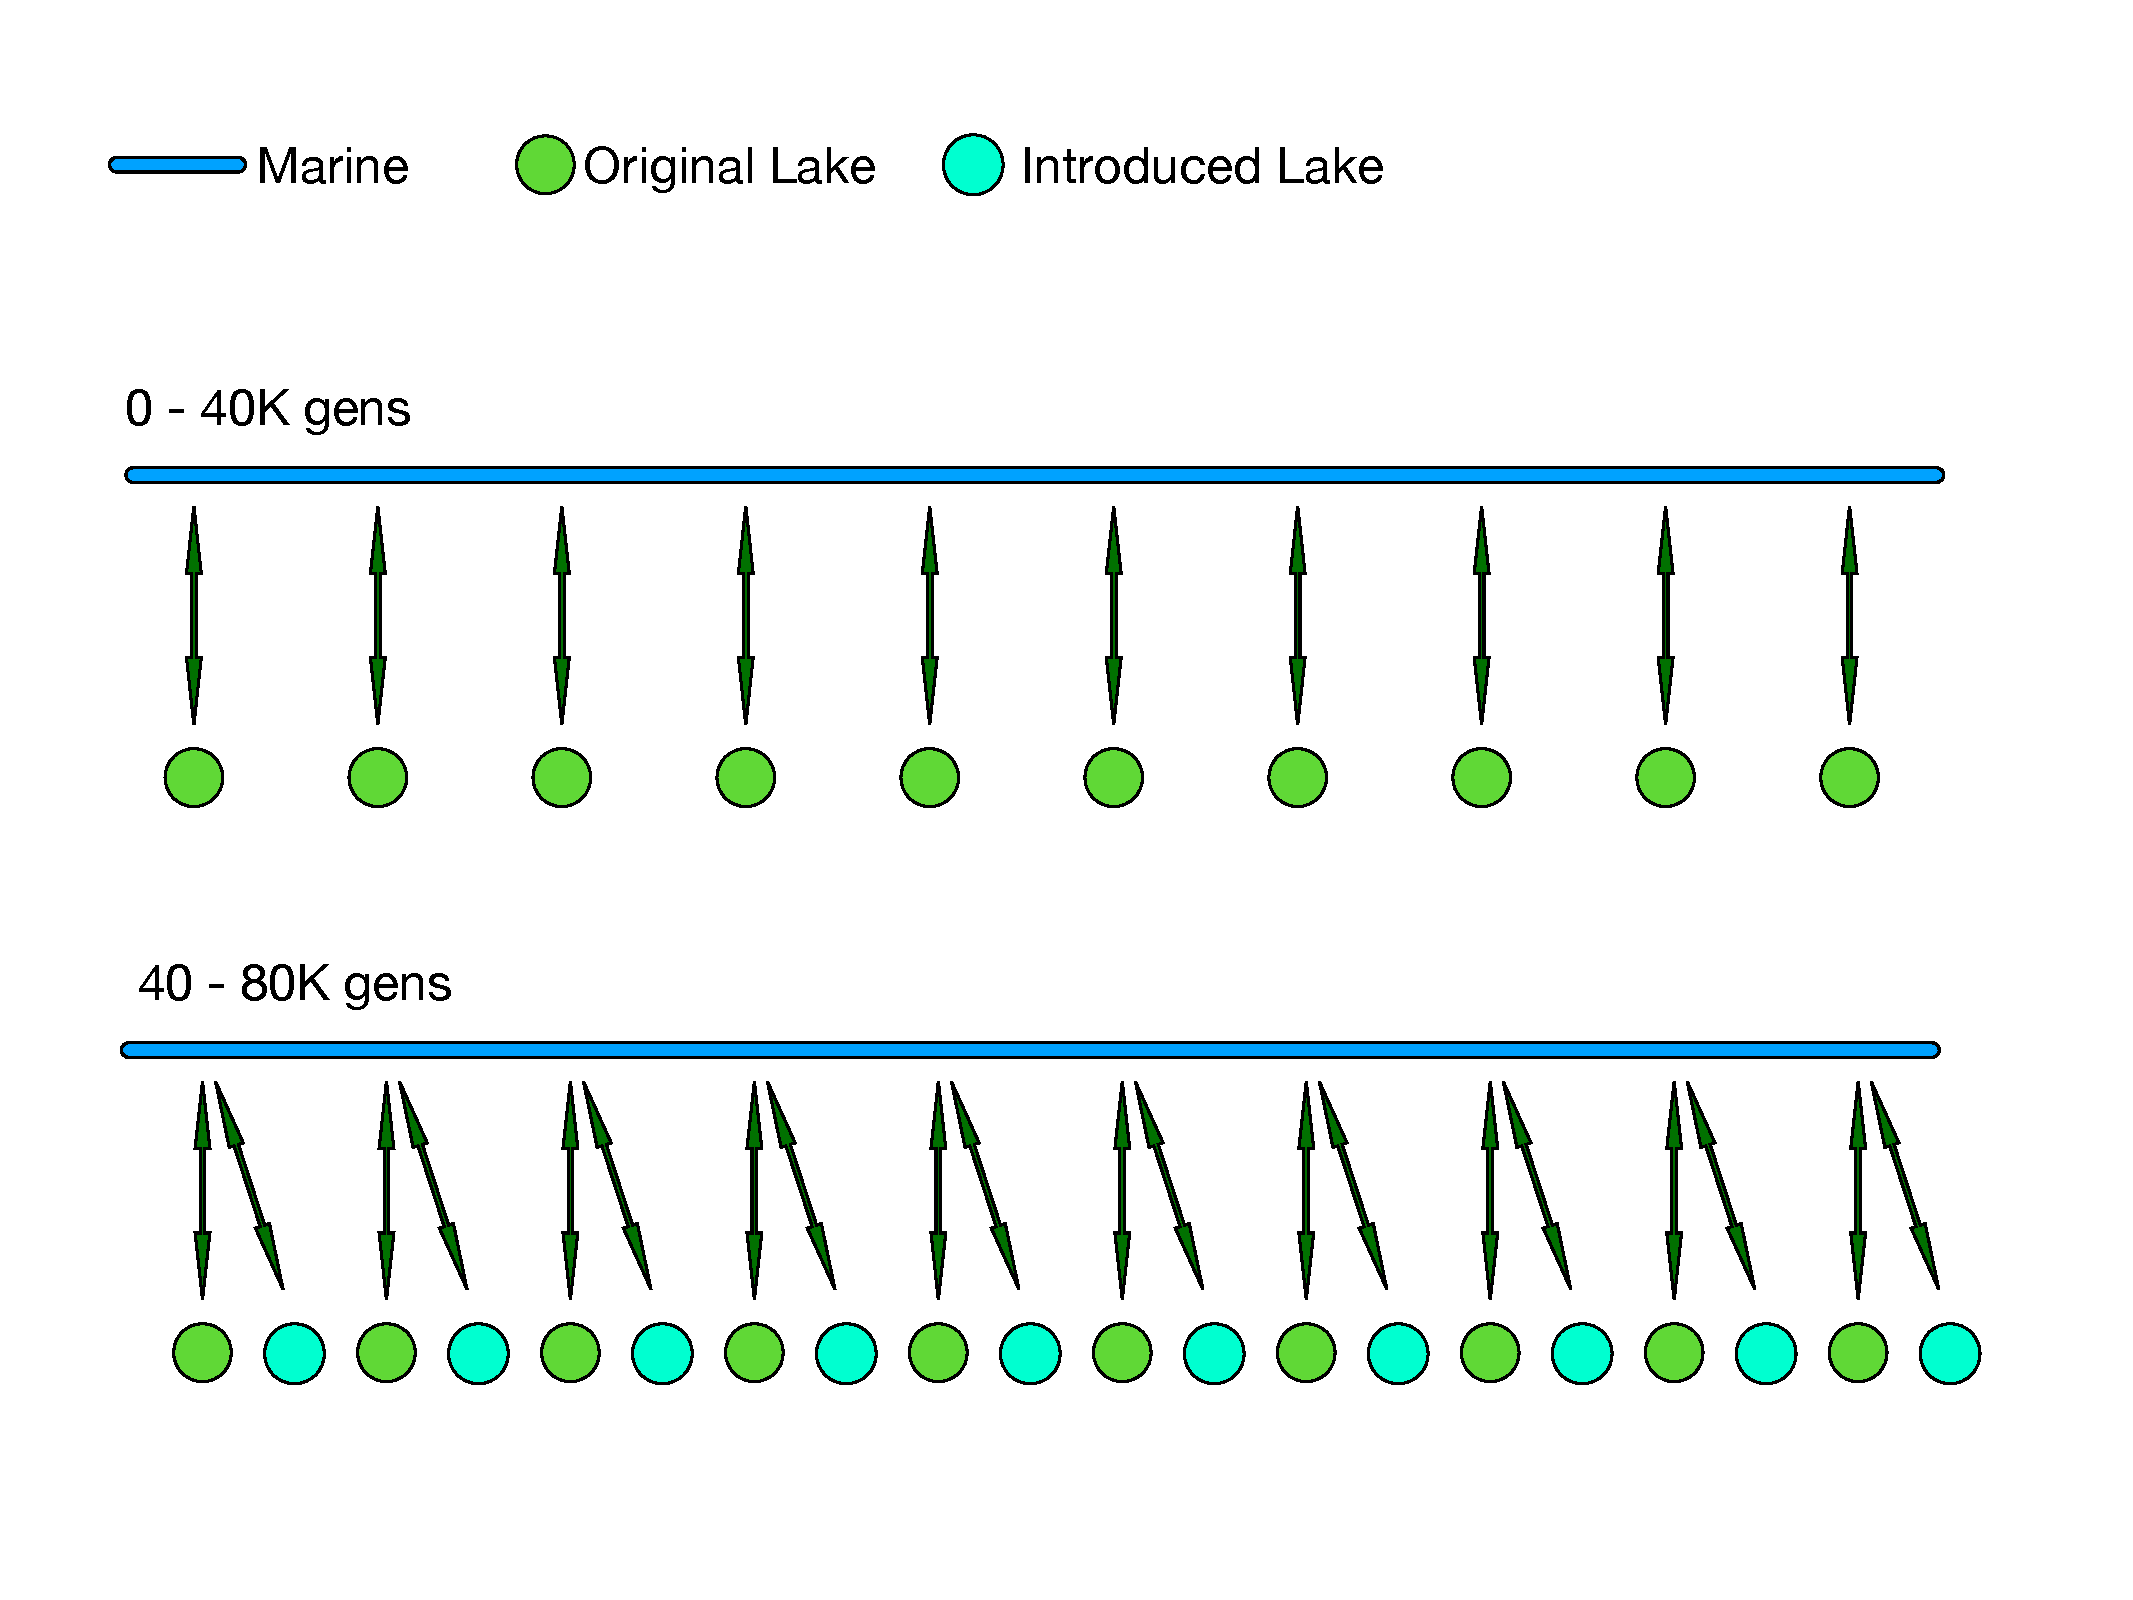
\includegraphics[width=0.8\linewidth]{GeographyDiagram}
  		\caption{A representation of the geographic and evolutionary history of all populations throughout the simulation. 
		The marine is a one-dimensional, continuous population with spatial positions ranging from [0.0 - 10.0]. Each 
		lake$_{i}$ is a discrete population connected by migration only through the marine at position $i - 0.5$. The introduced lakes 
		have the same location and selective pressure as the original lakes, but arise at 40K generations, 
		initialized as a copy of all marine individuals.}
  		\label{fig:Geo}
	\end{center}
\end{figure}

\subsubsection{Selective Pressure}

To emulate the freshwater and marine selective pressure, 
we set up a quantitative genetics model in which fitness is phenotypically based. 
Freshwater and Marine environments are distinguished by a single numeric value. 
This value is the optimum phenotype for each environment
and acts as a representation of lateral plate number and opercle shape in the stickleback populations.
The fitness of an individual is then determined by a probability density for a normal distribution 
at the quantile (?) of the difference between the optimum and the individual's phenotype


    \[
\textnormal{Individual.Fitness = } X \sim \mathcal{N}(\textnormal{Optimum - Individual.Phenotype},\,0.0\,15.0).
    \]

Where an individual?s phenotype is also defined by a single numeric value; 
determined as a summation of the selection coefficients of all mutations an individual possesses. 

	\[
{\textnormal{Individual.Phenotype = } \sum_{m \in mutations} \textnormal{m.selectionCoeff}}
	\]
    
\todo{This isn't quite right because of how we calculate additive, recessive, and dominant}
    
We allow six mutation types which affect phenotype along with one neutral mutation type.
Among the effect mutations; 
there are additive, dominant, and recessive mutations which effect phenotype
in either the positive or negative direction. 
The selection coefficients are pulled from a beta distribution 
with a shape parameter of $1$ and a mean of either $0.5$, or ${-0.5}$. 

	\[
\textnormal{Mutation.selectionCoeff = } X \sim \Gamma (1,\pm0.5)
	\]

\todo{maybe the order of these should be reversed?}

\subsubsection{Genomic Architecture}

Although still uncertain about how much of the genome is directly associated with the distinguished phenotypes, 
GWAS has indicated clusters of loci (linkage groups? Operon?) along the genome to be causative. 
To mimic this and compare dynamics of neutral vs. effect under selection, 
we create regions of effect. These genomic elements are the only loci which allow for mutation that impact phenotype. 
This allows us to observe differences in selection at the genomic level. 
In SLiM, the genome is conceptually a linear array of loci for which we can define
different amount 
\todo{finish this}


\subsection{Sampling}

%how did we use slim 
%More question based, Why did we measure what we measued 
%are there ways to have two or three subheaders 
%decriptive statist. 
%genetic basis -- 
%process of plotting. 
%if it's something new

Here, we're interested in observing how different parameter values
(mainly migrations rates and recombination rates)
impact the sharing of alleles between populations. 
we define freshwater adapted alleles (FAA),
at any given generation,
to be a mutations with a frequency higher than $0.5$ in \textit{any} of the original lakes, 
while remaining lower than $0.5$ in the marine. 
This is because the transportation hypothesis does not specify where or when an advantageous mutation arises; 
but simply suggests that when one comes to high enough frequency, it too, could participate in the transportation process. \cite{Schluter2009}
To observe transportation of freshwater alleles in our simulations, we use a variety of metrics when sampling.
Throughout the simulation, we measure;
mutation frequencies, 
$F_{st}$ values, 
average phenotype, 
mean number of original lakes each FAA appears in,
and total number of unique FAA. 
to understand where, as well as how much, of these freshwater haplotypes are being transported,
we track the mean percentage of FAA per individual (MPFAI) across all populations throughout the simulation:
computed as the sum of the FAA mutation frequencies among each population.
we're particularly interested in using MPFAI to measure the marine population' capacity to carry FAA,
as well as observing the introduced populations' ability to select upon them. 

Because we are interested in the local adaptation of the introduced freshwater populations,
we define time to adaptation ($T_{adapt}$) of the introduced population to be the generation at which
the difference between the average phenotype of the original and the introduced freshwater populations is less than 0.5. 
At this generation, we look at:
the correlation (B. Pearson) between the mutation frequencies of all effect loci and FAA,
and the number of shared high frequency alleles. 
These metrics tells us how much of the FAA  were used in the lakes once they have locally adapted. 


\section{Results}

%We found this
%--justify it

% A LIST OF PLOTS
% GENERAL OBSERVATIONS

% [1]. Fst Neutral 
% [2]. Fst Effect 
% [3]. Fst Across The 
% [4]. Median Number of FAA Per individual / Total Number of FAA
% [5]. Phenotype Distribution
% [6]. Percentage of shared High Frequency Alleles Shared Between Original and Introduced
% [7]. Correlation of Allele Frequency 
% [8]. Time until Adaptation
% [9]. Total Num FWAA - Average number of lakes each allele appears in.
% [10]. Distribution of # of FWAA Per marine individual.


\subsection{Local Adaptation: differentiation with gene flow}

Local adaptation occurred across all simulated parameter values.
Starting from the same baseline freshwater and marine populations diverged phenotypically, 
until they reached an equilibrium,
where the population means were close to or at the optimal phenotype. 
phenotypic variation within each population was small compared to the difference between populations.
Polymorphic loci that effected the phenotype,
showed greater differentiation compared to neutral loci between marine and freshwater populations, with the exception 
of migration rate at a value of $5e-5$. 
$F_{st}$ plots along the genome, show peaks at loci underlying local adaptation.

\todo{ add more general observations and caveats about not all parameter values. }


\subsection{The Effect of Migration Rate}

\subsubsection*{Migration is Mixing}

%FIGURES THAT SHOW THIS:
%- Fst Plots.
%- SGV Plots.
%- Haplotype plots

\begin{figure}[htb]
	\begin{center}
  		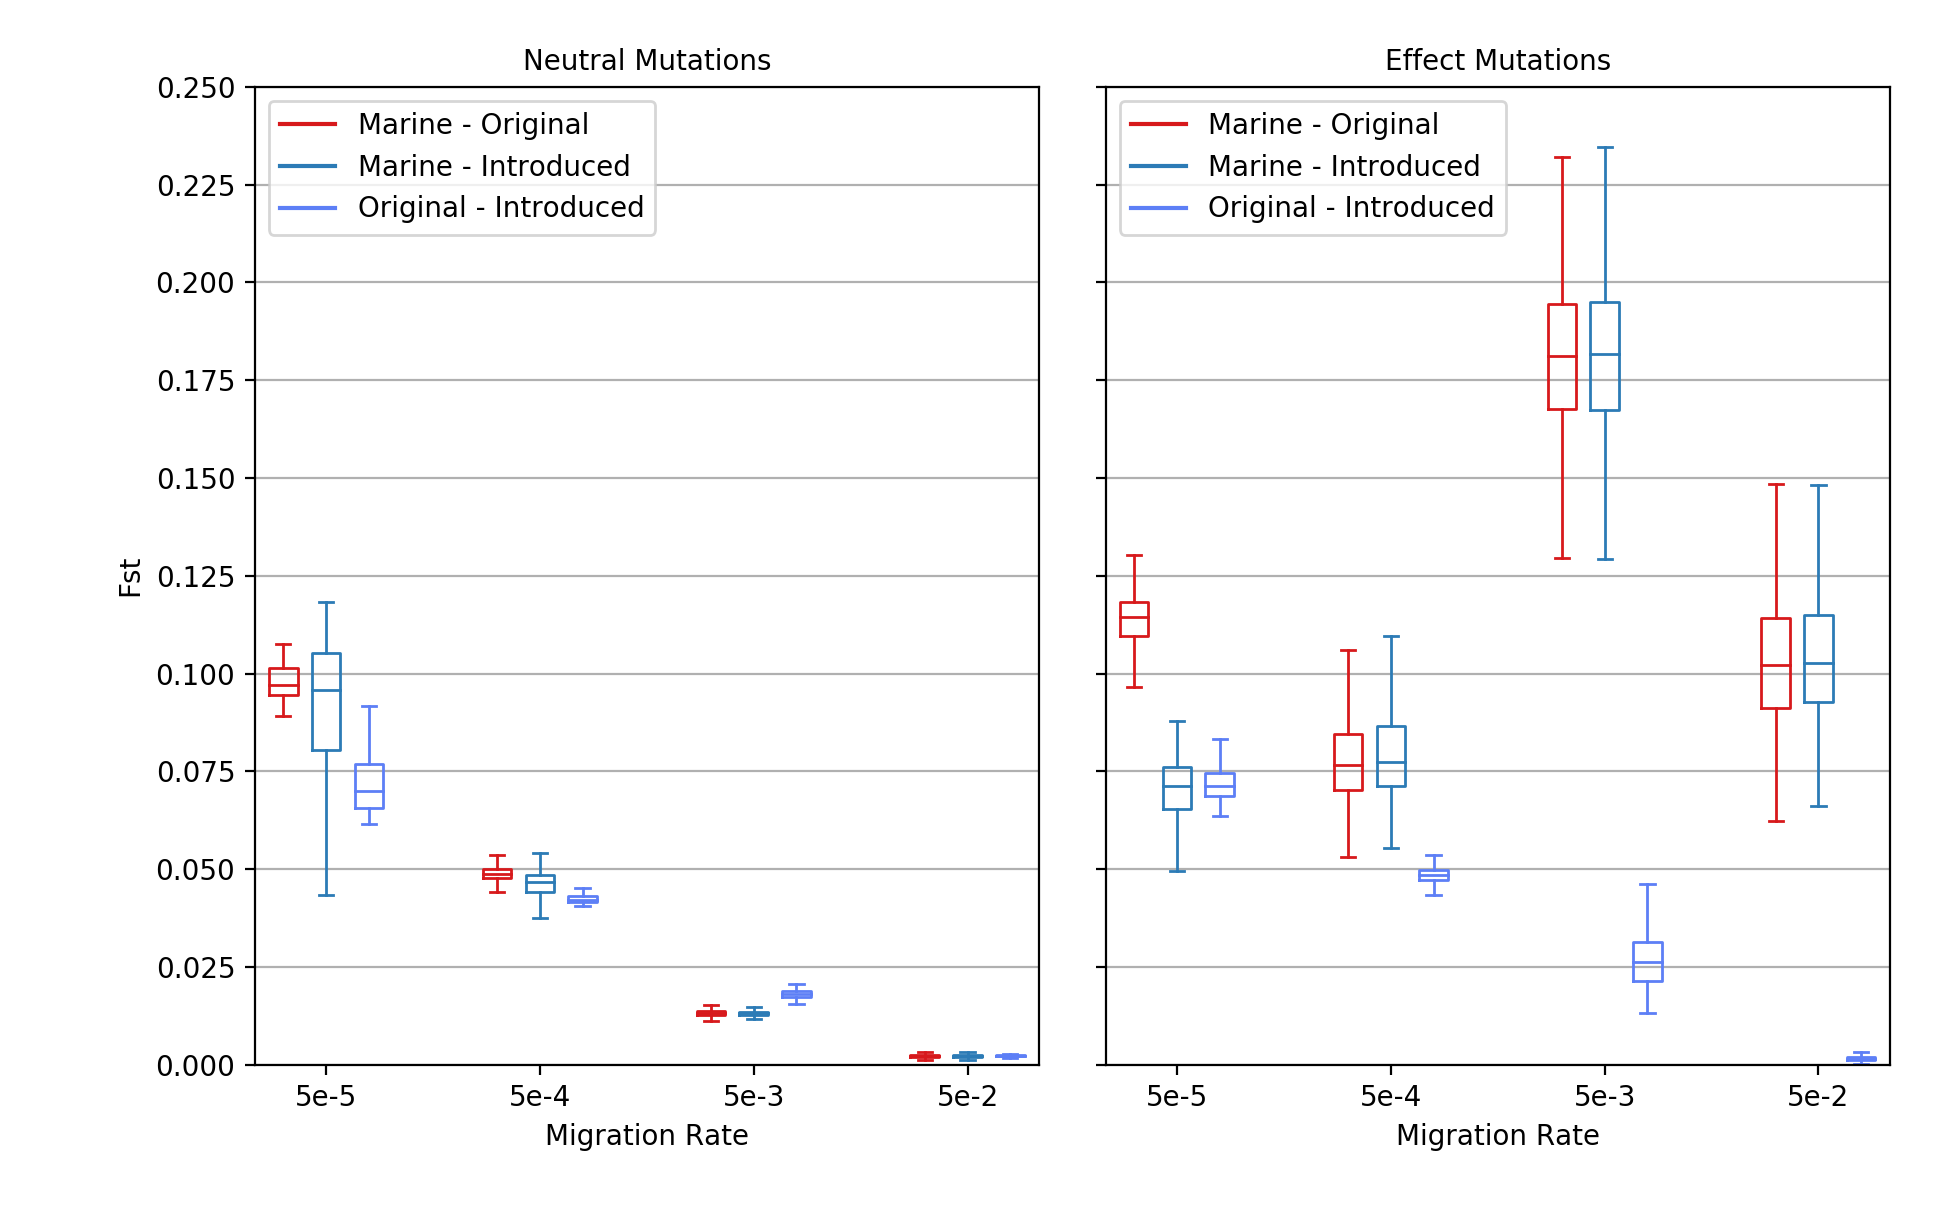
\includegraphics[width=01.0\linewidth]{matplotlib/Fst.png}
  		\caption{Distributions of $F_{st}$  values between the three subpopulations throughout the simulations.
		On the left, $F_{st}$ was calculated only on neutral mutation frequencies. On the right, $F_{st}$ was calculated
		only on effect (Impact on phenotype) mutation frequencies. 
		Effect mutations are acted upon by selection as they have an affect on fitness where neutral mutations  }
  		\label{fig:Fst}
	\end{center}
\end{figure}

Across increasing parameters of migration, we observed more gene flow across the populations. 
As can be seen in Figure \ref{fig:Fst},
$F_{st}$ values for neutral alleles steadily decline between all sets of populations as 
migration increases, this illustrates less difference between sections of the genome which are not acted up 
upon by selection, in all populations.
Additionally, Standing Genetic Variance \todo{computed as?}
(Seen in SGV Figure)
values in the marine population steady increased with migration which suggests that more alleles from the 
lakes surrounding were exporting alleles into the marine individuals.
\todo{Something about SGV rates for the the other population}

%TIES TO NATURE?
%SPECIFICALLY (interesting stuff)

\subsubsection*{migration affects the speed of adaptation}

%FIGURES THAT SHOW THIS:
%-Time to adaptation
\begin{figure}[h!tb]
	\begin{center}
  		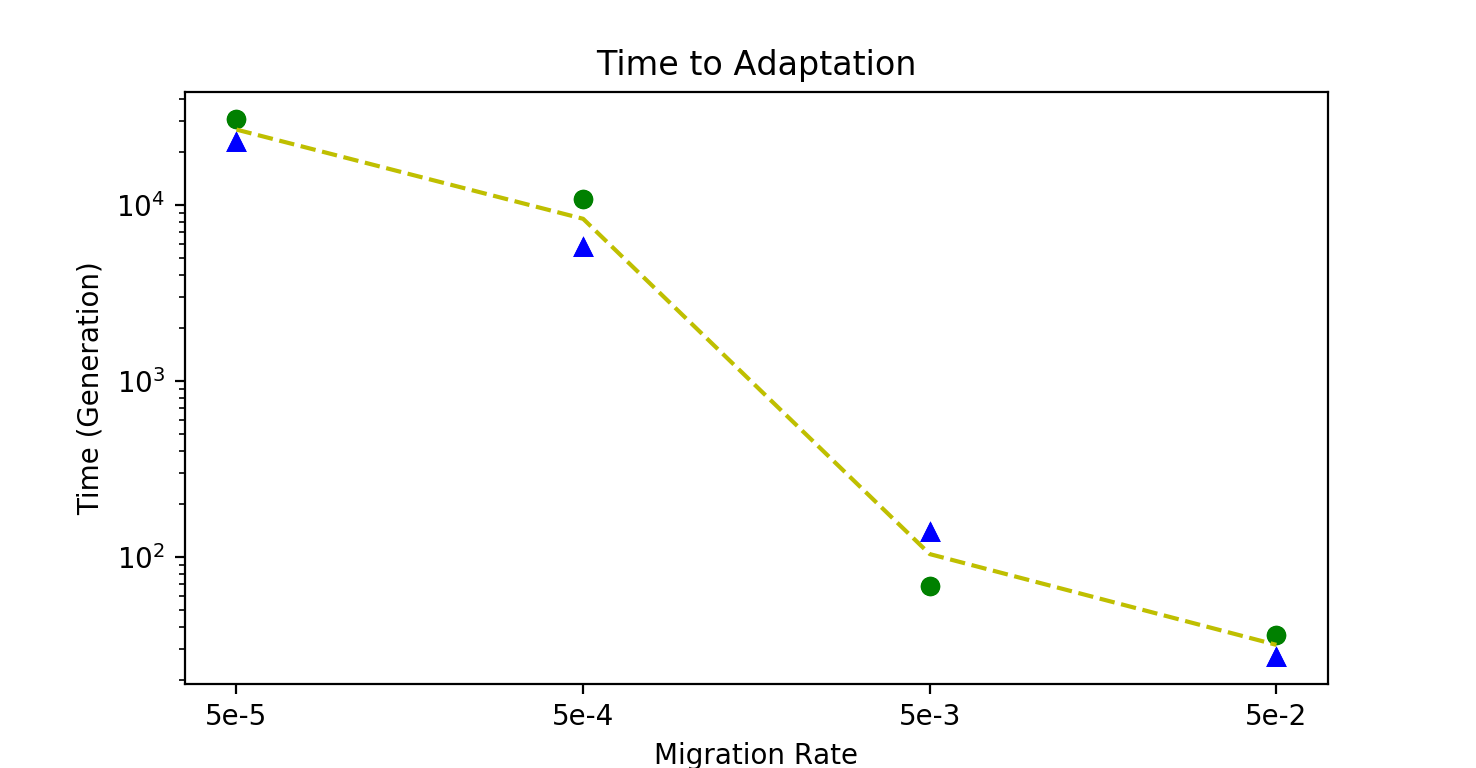
\includegraphics[width=01.0\linewidth]{matplotlib/TimeToAdaptation.png}
  		\caption{Time to adaptation as a function of migration rate ($M$) parameter value. This is where we measure how many generation
		it takes for the introduced population's mean phenotype to come within 0.5 of the original lakes average phenotype. 
		Each point represents a simulation run at some value of $M$. 
		The yellow dashed line is the average of all points at each respective parameter value}
  		\label{fig:TimeToAdaptation}
	\end{center}
\end{figure}

We observed a dramatic shift in time until adaptation for the introduced populations
as migration rates increased. 
As can be seen in Figure \ref{fig:TimeToAdaptation} at the lowest migration rate of $5 * 10^{-5}$,
It took the introduced population over 30 thousand generations for the average phenotype of all the lakes to 
get to within 0.5 of the original lakes original phenotypes. 
This suggests that selection was acting primarily on new mutations, meaning the 
introduced lakes needed to wait for a beneficial mutation to arise before 
it was selected upon. 
There was a positive correlation between the amount of standing genetic variation in the 
marine and the rapid adaptation of the introduced populations.

%TIES TO NATURE?
 
\subsubsection*{sharing of freshwater adapted alleles}

%FIGURES THAT SHOW THIS:
%-MPAA / IND
%-Total/Avg shared
\begin{figure}[h!tb]
	\begin{center}
  		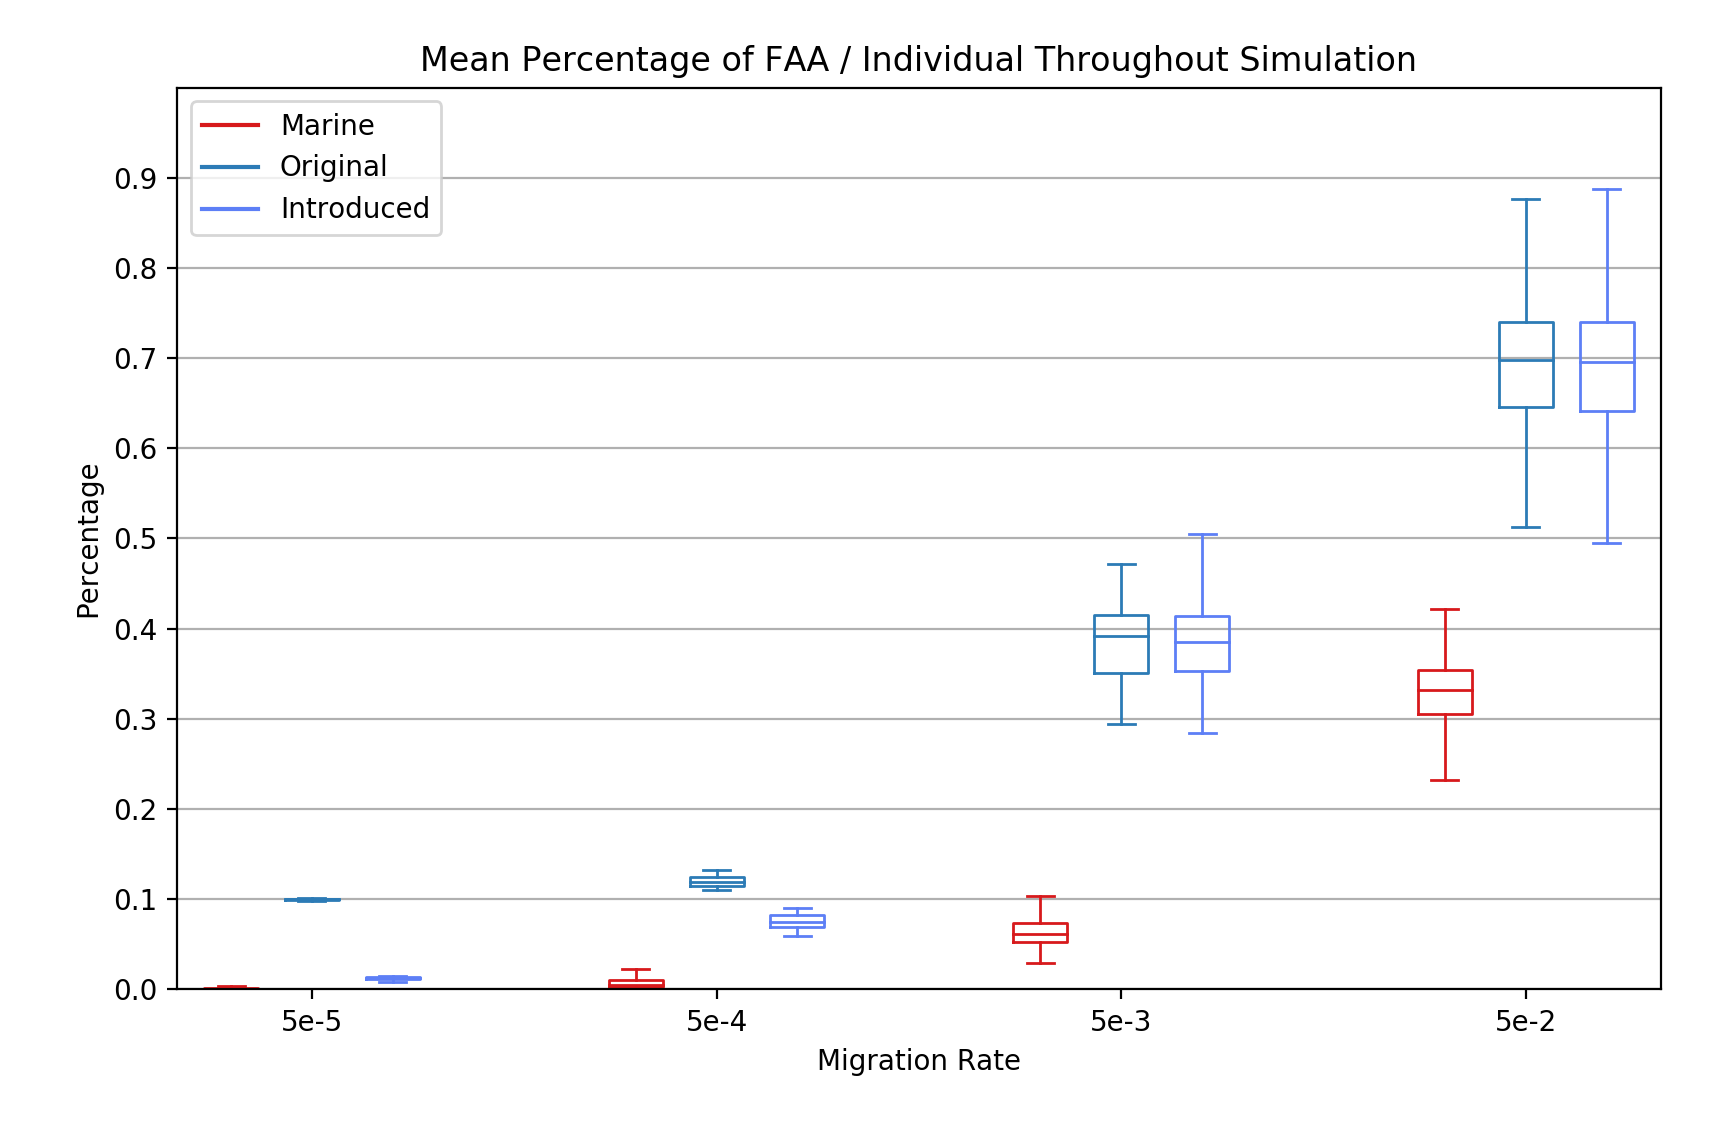
\includegraphics[width=0.8\linewidth]{matplotlib/MPFAI.png}
  		\caption{Distributions of mean percentage of freshwater adapted alleles (FAA) throughout the simulation run, for each subpopulation.
		We count the total number of freshwater alleles for each individual before averaging them in each population and dividing by the total number of defined
		freshwater adapted alleles.
		Looking at total number of FAA per individual gives us an idea behind how many alleles underly a freshwater haplotype, 
		while the percentage tells us the variance of the haplotype (note: I also have boxplots telling us total num FAA for the average individual that are interesting to look at "matplotlib/MFAI.png")}
  		\label{fig:MPFAI}
	\end{center}
\end{figure}



To further investigate this correlation, we take a look at the FAA driving 
local adaptation of the introduced population. 
One common metric we investigate is the percentage of FAA per individual in each of the populations. 
This gives us a general look at the where these alleles are being distributed. 
Looking at the lowest migration rate for the original lakes population In Figure (MPAA / IND) 
We see that the average individual has almost exactly $1/10^{th}$ of the total defined FWAA throughout the simulation. 
Because FAA are defined among \textit{any} population, this suggests that each one of the $10$ 
lakes has created their own solution to adaptation of the the freshwater selective pressure. 

As we can see in Figure (Total/Avg shared)
as migration rate parameter increases for the simulations, 
we see the distribution of the total number of FAA's decrease, and 
the average number of lakes each allele appears in at high frequency ($p > 0.5$), increase.
With the distribution of effect size remaining the same across all simulations, 
these are both suggestive of the original lakes sharing solutions to the same selective pressure.

%TIES TO NATURE?

%SPECIFICALLY (interesting stuff)

\subsubsection*{We see Migration Load after a certain threshold of migration}

%FIGURES THAT SHOW THIS:
%- Phenotype Distribution
\begin{figure}[h!tb]
	\begin{center}
  		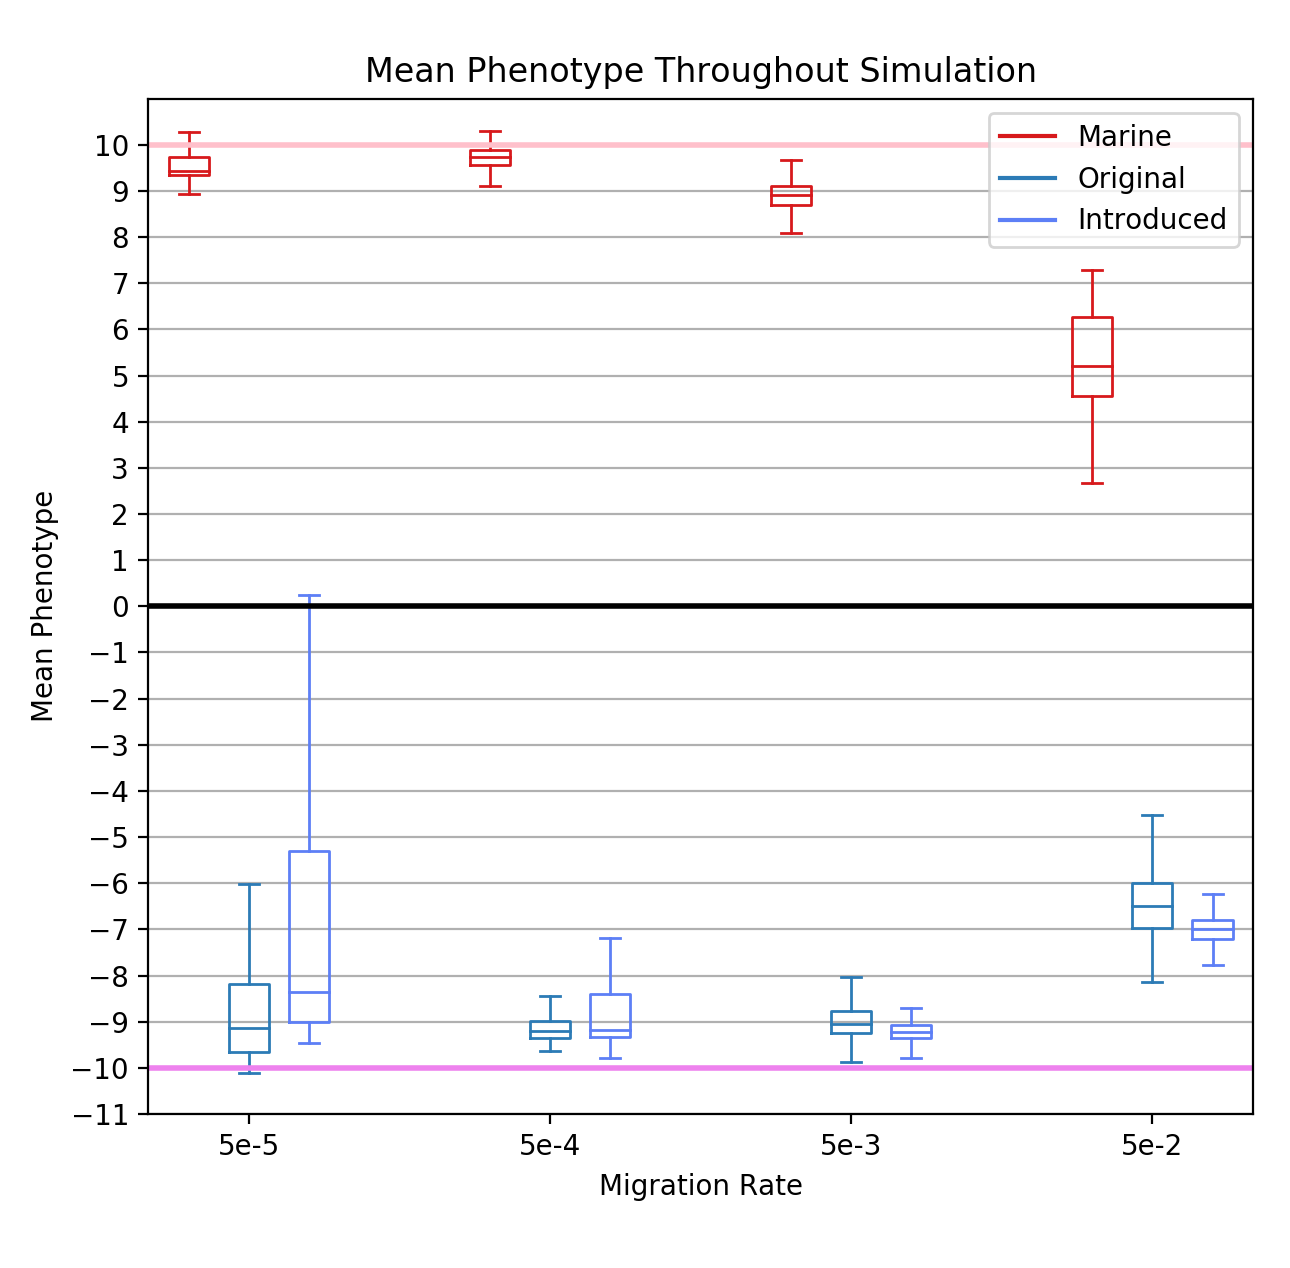
\includegraphics[width=0.8\linewidth]{matplotlib/MeanPhenotype1.png}
  		\caption{Distribution of mean phenotype throughout simulation runs at separate migration rate ($M$) parameter values, for each population.
		The dashed pink line (Pheno = +10) is the optimum phenotype any individual in the marine environment.
		In contrast the purple line at (Pheno = -10) represents the optimum for any individual in the freshwater environment. 
		All individuals at generation 0 (beginning of the simulation) 
		}
  		\label{fig:MeanPhenotype}
	\end{center}
\end{figure}

%GENERAL

In the distributions we have shown across migration rate parameter values, 
We have experienced the most dramatic shifts of the population dynamics at $M = 5x10^{-3}$.
After a threshold between this and $M = 5x10^{-2}$, we start to experience migration load. 
Significant gene flow constricts local adaptation
as a consequence of a large number of offspring through hybridization events between subpopulations.
In Figure \ref{fig:MeanPhenotype} at $M = 5x10^{-2}$, we can see the distribution of average phenotype throughout the simulation
pull towards the opposing selective pressure value and away from the local optimum in all subpopulations.


%TIES TO NATURE?

%SPECIFICALLY (interesting stuff)
	
\subsubsection*{There is a Qualitative Threshold of migration rates}

%FIGURES THAT SHOW THIS:
%all
%TIES TO NATURE?
%SPECIFICALLY (interesting stuff)

%GENERAL
We have found that too little migration leads to selection upon new mutations in all subpopulations and lakes alike. 
In contrast, at high migration rates we have seen that migration load limits 
the ability for species to locally adapt to the selective pressure of their environment.
This leads us to consider a window (Goldilocks Zone) of introgression which allows for the transportation
of FAA's without migration load. In a species that commonly is subjected to two general types of selective pressure 
such as marine and 

\subsubsection*{Low Recombination Causes Clustering}

\begin{comment}
%--------------------------------------------------------------------------------------------------------------------------------------------------------------------------------------------
%SHOULD PROBABLY JUST DELETE ALL THIS. V UNORGANIZED.
Across migration rates we observe a large difference in:
gene flow, 
$F_{st}$ values,
amount of time until adaptation,
sharing of solutions (haplotytes?),
$SGV$,
and, migration load. 
we run multiple simulations across a range of migration rates starting at $5e-5$ and increasing by
one order of magnitude up to $.05$. 
With the marine and freshwater both at a population size 2000,
this represents exactly $1/10_{th}$, $1$, $10$, and $100$ migrants per generation, respectively. 

At low migration rates of $5e-5$ (1/10 migrants per generation), we observed little sharing of genetic solutions and 
almost no freshwater alleles existing in the marine population.
With an MPFAI of $0.0999$ in the original lakes;
each individual in the original lakes had almost exactly $1/10_{th}$ of the total FAA. 
In addition to each allele appearing in an average of $1.08$ lakes, 
this tells us that each of the 10 lakes has individually selected their own set of solutions (haplotypes) 
rather than sharing alleles through the marine. 
This is further supported by the low capacity of the marine to transport the alleles with an MPFAI of $0.003$.
$T_{adapt}$ remained on an ecological timescale of $18K$ generations, and the correlation of FAA frequencies was at $0.09$.
With the introduced population having an MPFAI of $0.02$, 
we see little evidence that the lakes were able the select on the alleles found in that marine. 
it may be important to note that while we are sampling the 10 introduced lakes as a whole population,
It is possible that only a couple of the lakes even received a copy some alleles during the introduction.
However, to see evidence of the haplotypes being carried throughout the marine we would expect to observe a pattern off all lakes
being able to select upon similar alleles. 
This observation gives a migration rate below the threshold needed to support the transportation hypothesis.

scaling up migration rates to $0.0005$ (1 migrants per generation)
we observe the first evidence of transportation.
The mean total number of FAA drops to 45 and the average number of lakes which each alleles appears in jumped to $1.33$. 
This shows us the gene flow between populations allowed for some freshwater alleles to travel through the marine and be shared by the lakes. 
Interestingly, with the marine showing an MPFAI of $0.02$, 
the introduced was much more able to select upon the alleles;
The introduced population showed a MPFAI of $0.078$, compared to the original lakes which was at $0.129$,
Looking at the FAA frequencies in the two freshwater populations at time of adaptation, we see a correlation of $.68$
While this is evidence of parallel local adaptation, the  $T_{adapt}$ was still at $8,365$ generations.

At $0.005$ (10 migrants per generation) we experience high correlation between the FAA frequencies
in the original and introduced populations, $0.96$, and rapid local adaptation of the introduced population, (81 generations). 
With the introduced population showing an MPFAI of  ~ $0.34$ which is strikingly close to the original freshwater population which is at $0.34$
This migration rate clearly shows the capacity to share alleles in order for us to see rapid and parallel adaptation.
 
Interestingly, is that if we look at the distribution and total amount of FAA in the marine population at time of introduction between 
$0.0005$ and $0.005$, they are virtually identical.
This comes with two questions
(1) why is there a similar amount of FAA in the marine with such a substantial difference in migration, and
(2) what is it about the higher migration rate of  $0.005$ that allows it perform so much better in terms of rapid adaptation? 
To answer the first question we can see that the median number of defined FAA is much higher, 45
While with the higher migration there is only a median of 10. 
This is a result of the solutions not being shared across the original lakes at lower migration rates.
This can be seen by the average number of lakes each FAA appears in being 
$1.54$ at 1 migrant per generation and 
$3.75$ at 10 migrants per generation.
consequently more alleles were defined as FAA and sampled as such in the marine population. 
This however does not explain why, at higher migration rates, 
the introduced freshwater population was able to rebuild the haplotype so much more quickly. 
For this, It is important to note that after introduction, there is continued migration. 
This means that for a migrate of $0.005$ there is roughly 10 times as 
much of the FAA being brought into the freshwater every generation compared to migrate $0.0005$.

This seams to suggest that continued migration is quite important 
for rapid adaptation at this migration rate as opposed to the simply the concentration of 
freshwater adapted alleles found in the marine. 

Note: we should probably investigate the distribution of effect size more to clearly answer the above questions ...

(NOTE:PETER/BILL how does this compare to what we see in nature


\subsection{Qualitative Threshold}

\subsection{Migration Load}

%\begin{figure}
%	\begin{center}
%  		\includegraphics[width=1.2\linewidth]{MigrationLoad}
%  		\caption{A boat.}
%  		\label{fig:boat1}
%	\end{center}
%\end{figure}

While both of the higher migration rates of $0.005$ and $0.05$ showed evidence of sharing alleles and rapid adaptation,
we see substantial difference in the median phenotype compared to the optimum for each subpopulation. 
This is because migration tends to oppose the natural divergence of populations undergoing ecological speciation. \cite{Bolnick}
Migration load depreciation of fitness between two subpopulations with a high amount of introgression between them. 
This is often observed in nature when the sharing of genes constricts the adaptation of both species. 

In our simulations, at high migration rates of $0.05$, 
we consistently saw this effect in all subpopulations. 



\subsection{Low Recombination in Effect Regions}

Goldilocks Zone? 

at 10 migrants/generation (or 0.005 of the population) 
is the first parameter value at which we observe 

%--------------------------------------------------------------------------------------------------------------------------------------------------------------------------------------------
\end{comment}

\section{Conclusion \& Discussion}

% at low M we should be able to predict something ---
% at high M we should be able to predict something ----

Here, we suggest a range of migration rate (introgression) parameter values which would allow for the rapid (and in turn, parallel) adaptation 
of marine stickleback introduced intro a freshwater environment.
While this range is heavily effected by all other selections of parameter values. 

\newpage
\bibliography{Citations}{}
\bibliographystyle{plain}



\end{document}